\begin{figure}[t]
\centering
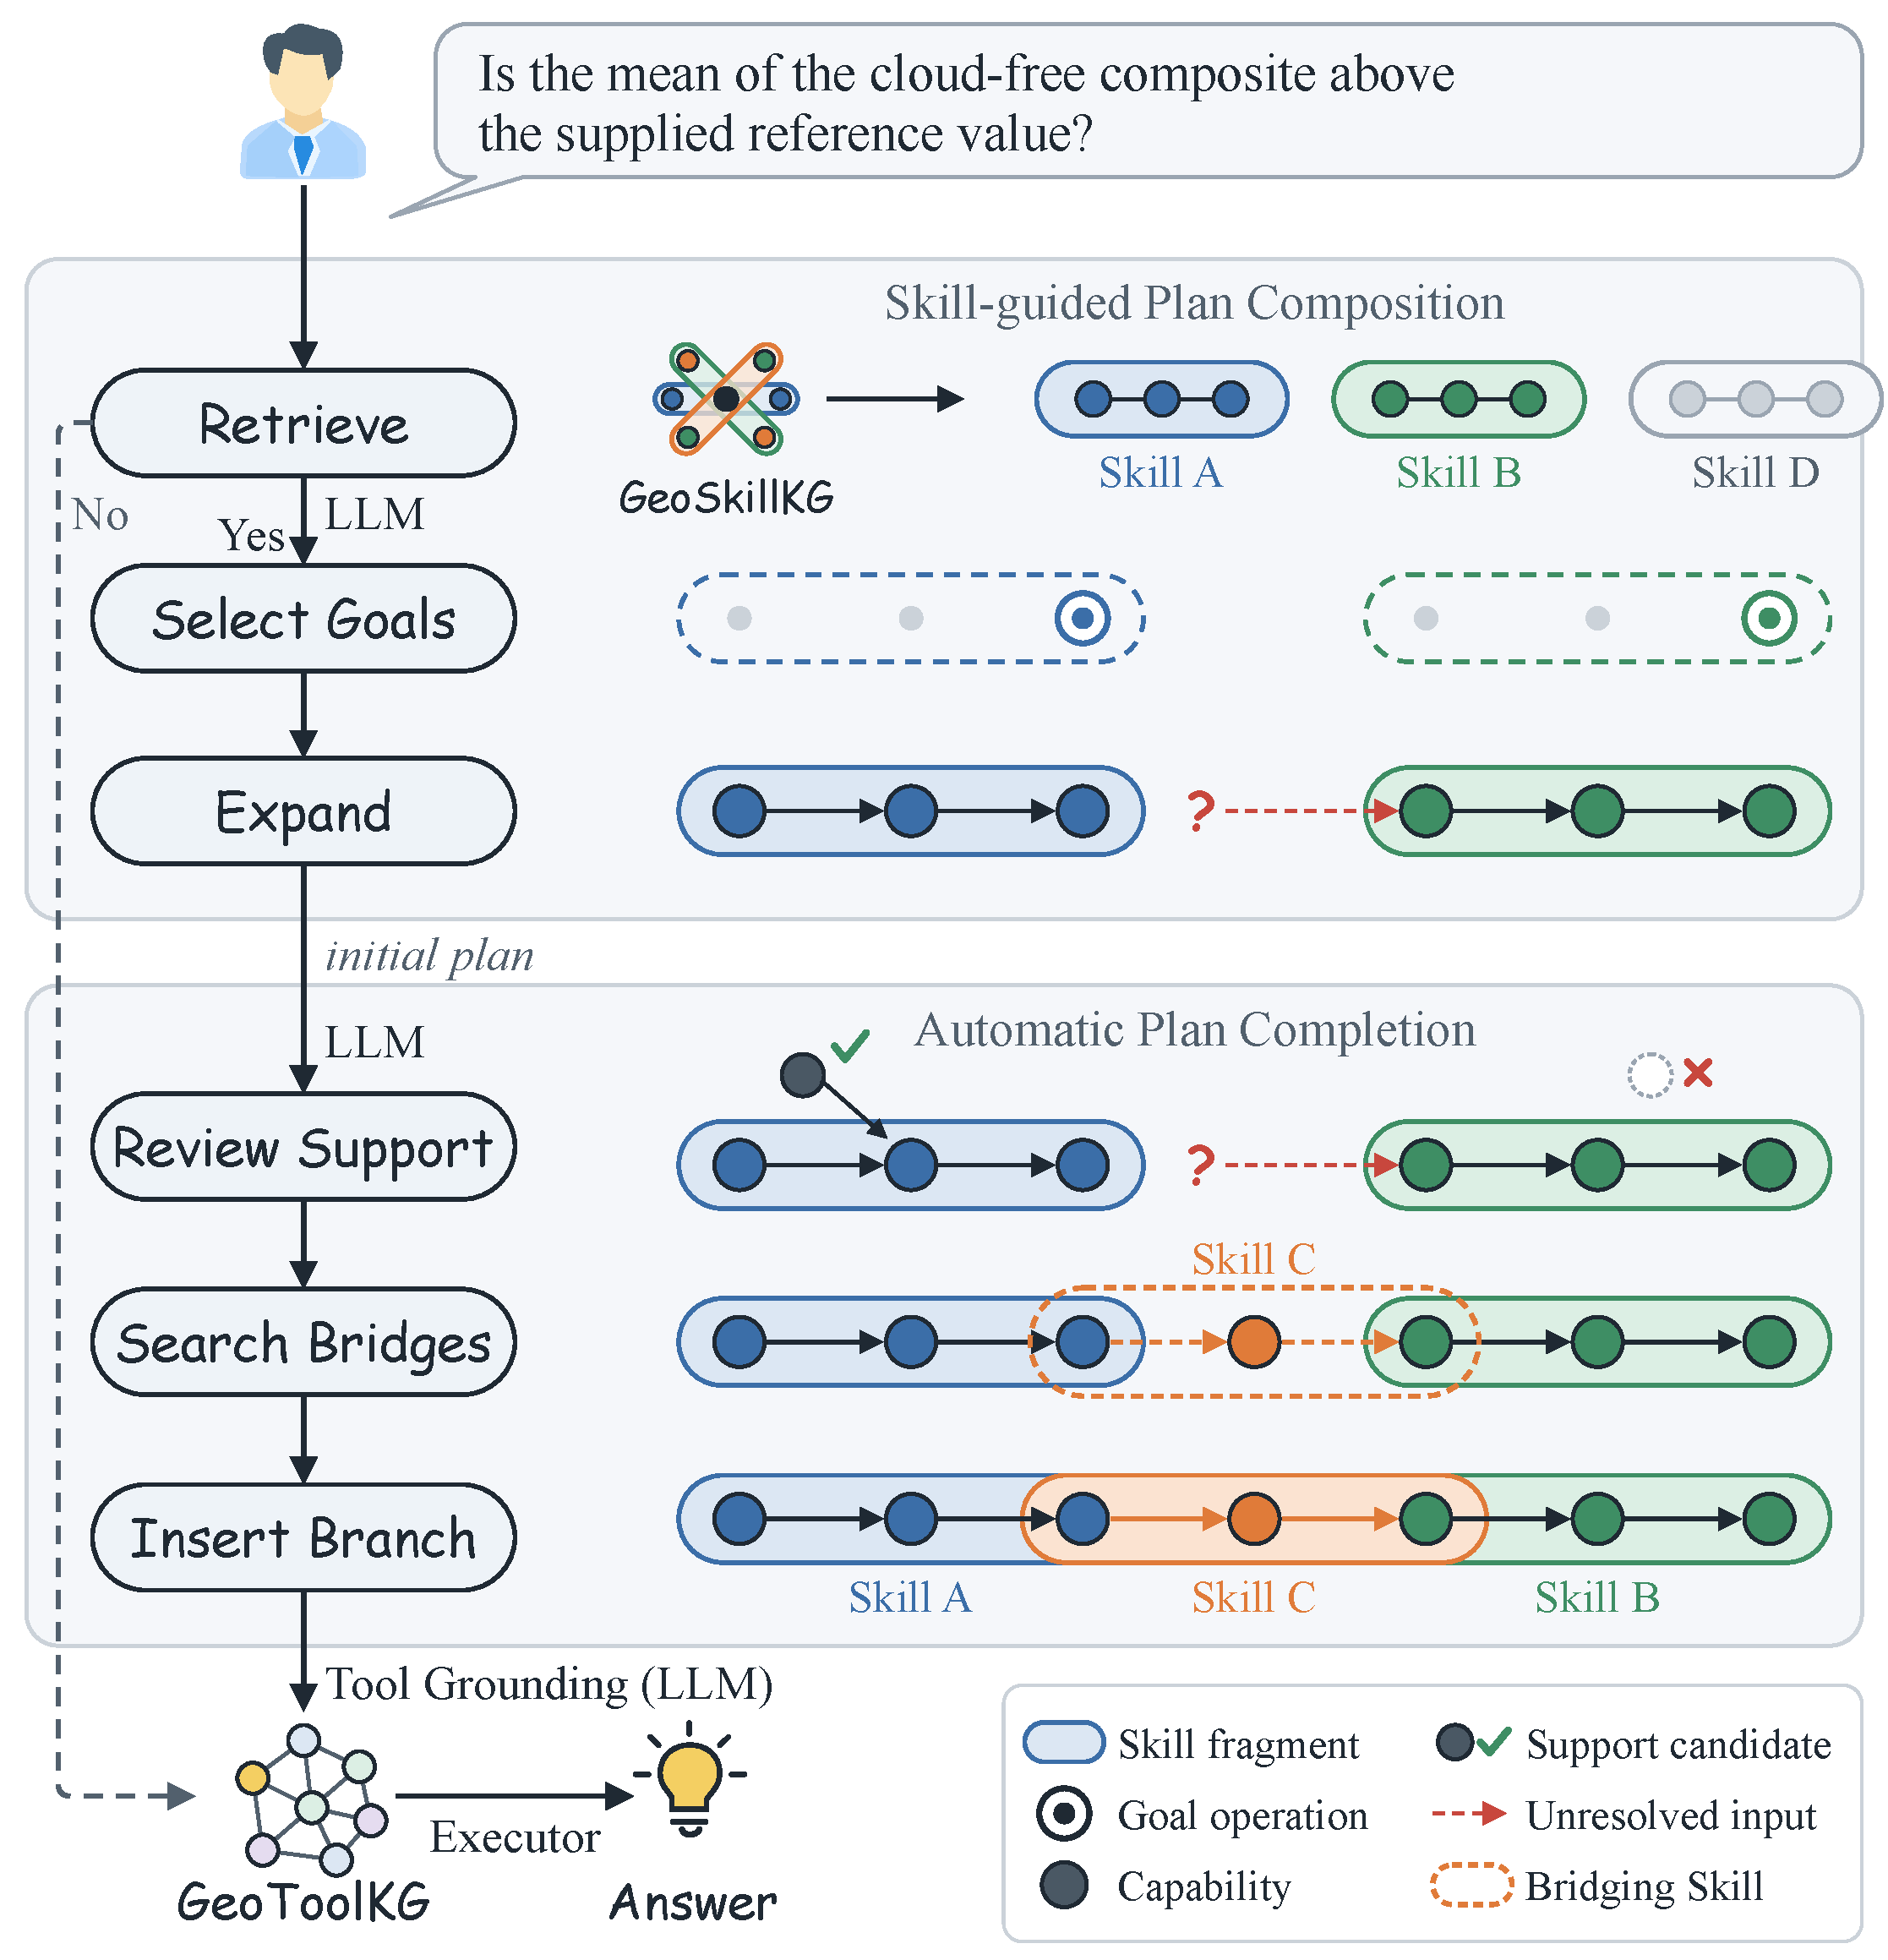
\includegraphics[width=\columnwidth]{fig_pipeline.pdf}
\caption{AgentGS planning pipeline. Composition turns retrieved Skills into an initial plan; completion inserts a bridging branch from another Skill to resolve an open input. Without an applicable Skill, planning falls back to the tool-only path.}
\label{fig:pipeline}
\Description{A vertical flowchart. Pills on the left list the stages Retrieve, Select Goals, Expand, Review Support, Search Bridges, and Insert Branch, grouped into Skill-guided Plan Composition and Automatic Plan Completion. Beside each stage a thumbnail shows the plan: retrieved Skills A, B, and D; goal operations of A and B; expanded fragments with an unresolved input; an accepted and a rejected supporting operation; Skill C bridging the fragments; and the completed chain A, C, B. The plan is then grounded over GeoToolKG and executed to produce the answer. A dashed path leads from Retrieve directly to GeoToolKG when no Skill applies.}
\end{figure}
